\let\negmedspace\undefined
\let\negthickspace\undefined
\documentclass[journal]{IEEEtran}
\usepackage[a5paper, margin=10mm, onecolumn]{geometry}
%\usepackage{lmodern} % Uncomment if needed for pdflatex


\setlength{\headheight}{1cm} % Set the height of the header box
\setlength{\headsep}{0mm}     % Set the distance between the header box and the top of the text

\usepackage{gvv-book}
\usepackage{gvv}
\usepackage{cite}
\usepackage{amsmath,amssymb,amsfonts,amsthm}
\usepackage{algorithmic}
\usepackage{graphicx}
\usepackage{textcomp}
\usepackage{xcolor}
\usepackage{txfonts}
\usepackage{listings}
\usepackage{enumitem}
\usepackage{mathtools}
\usepackage{gensymb}
\usepackage{comment}
\usepackage[breaklinks=true]{hyperref}
\usepackage{tkz-euclide} 
\usepackage{listings}
%\usepackage{gvv}                                        
\def\inputGnumericTable{}                                 
\usepackage[latin1]{inputenc}                                
\usepackage{color}                                            
\usepackage{array}                                            
\usepackage{longtable}                                       
\usepackage{calc}                                             
\usepackage{multirow}                                         
\usepackage{hhline}                                           
\usepackage{ifthen}                                           
\usepackage{lscape}
\usepackage{tikz}
\usepackage{circuitikz}
\usepackage{standalone} % For including external TikZ files

\begin{document}

\bibliographystyle{IEEEtran}
\vspace{3cm}

\title{10.4.ex.8}
\author{EE24BTECH11013 - MANIKANTA D}
% \maketitle
% \newpage
% \bigskip
{\let\newpage\relax\maketitle}

\renewcommand{\thefigure}{\theenumi}
\renewcommand{\thetable}{\theenumi}
\setlength{\intextsep}{10pt} % Space between text and floats

\numberwithin{equation}{enumi}
\numberwithin{figure}{enumi}
\renewcommand{\thetable}{\theenumi}
\textbf{Question}:\\
Find the roots of the equation $5x^2 - 6x - 2 = 0$ by the method of completing the square.
\textbf{Solution:} Multiplying the equation throughout by $5$, we get
\begin{align}
25x^2 - 30x - 10 = 0.
\end{align}
This is the same as
\begin{align}
(5x)^2 - 2 \cdot (5x) \cdot 3 + 3^2 - 3^2 - 10 = 0, \\
(5x - 3)^2 - 9 - 10 = 0, \\
(5x - 3)^2 - 19 = 0, \\
(5x - 3)^2 = 19.
\end{align}
Taking the square root on both sides, we get
\begin{align}
5x - 3 = \pm \sqrt{19}, \\
5x = 3 \pm \sqrt{19}, \\
x = \frac{3 \pm \sqrt{19}}{5}.
\end{align}
Therefore, the roots are
\begin{align}
x = \frac{3 + \sqrt{19}}{5} \quad \text{and} \quad x = \frac{3 - \sqrt{19}}{5}.
\end{align}
\textbf{QR decomposition on Hessenberg matrix:}\\
The QR decomposition method is a numerical algorithm to compute the eigenvalues of a matrix $A$. By iteratively factorizing the matrix $A$ into the product of an orthogonal matrix $Q$ and an upper triangular matrix $R$, and then recombining them in a specific order, the process converges to a diagonal matrix whose diagonal entries are the eigenvalues of $A$.

This document adapts the QR decomposition method specifically for finding the roots of the quadratic equation $5x^2 - 6x - 2 = 0$.

\textbf{QR Decomposition for Quadratic Roots}:
Given the quadratic equation $5x^2 - 6x - 2 = 0$:

\begin{enumerate}
    \item Rewrite the equation in matrix form. For a quadratic equation $ax^2 + bx + c = 0$, the companion matrix is:
    \[
    A = \begin{bmatrix}
    0 & 1 \\
    -\frac{c}{a} & -\frac{b}{a}
    \end{bmatrix}.
    \]
    For $5x^2 - 6x - 2 = 0$, this becomes:
    \[
    A = \begin{bmatrix}
    0 & 1 \\
    -\brak{\frac{-2}{5}} & -\brak{\frac{-6}{5}}
    \end{bmatrix} = \begin{bmatrix}
    0 & 1 \\
    \frac{2}{5} & \frac{6}{5}
    \end{bmatrix}.
    \]

    \item Perform the QR decomposition of $A$:
    \begin{align}
    A_n = Q_n R_n,
    \end{align}
    where $Q_n$ is an orthogonal matrix and $R_n$ is an upper triangular matrix.

    \item Update the matrix:
    \begin{align}
    A_{n+1} = R_n Q_n.
    \end{align}

    \item Repeat steps 2 and 3 until $A_n$ converges to an upper triangular matrix. The diagonal elements of this matrix are the eigenvalues, which correspond to the roots of the quadratic equation.
\end{enumerate}

\textbf{Mathematical Description}:
At the $n$-th iteration, let $A_n$ be the matrix:
\begin{align}
A_n = Q_n R_n,
\end{align}
where $Q_n$ and $R_n$ are obtained via the QR decomposition of $A_n$. The matrix is updated as:
\begin{align}
A_{n+1} = R_n Q_n.
\end{align}

\textbf{Update Equation}:
The update equation for the $(n+1)$-th iteration in terms of the $n$-th iteration is:
\begin{align}
A_{n+1} = Q_n^T A_n Q_n,
\end{align}
where $Q_n$ is the orthogonal matrix from the QR decomposition of $A_n$, and $R_n$ is an upper triangular matrix such that $A_n = Q_n R_n$.

\textbf{Roots of the Quadratic Equation}:
The eigenvalues of the companion matrix $A$ correspond to the roots of the quadratic equation $5x^2 - 6x - 2 = 0$. As the iterations progress, the diagonal elements of $A_n$ will converge to the roots of the equation. The algorithm involves the following steps:
\begin{enumerate}
    \item Initialize $A_0$ as the companion matrix:
    \[
    A_0 = \begin{bmatrix}
    0 & 1 \\
    \frac{2}{5} & \frac{6}{5}
    \end{bmatrix}.
    \]

    \item Perform the QR decomposition of $A_n$:
    \begin{align}
    A_n = Q_n R_n,
    \end{align}
    where $Q_n$ is orthogonal and $R_n$ is upper triangular.

    \item Compute $A_{n+1}$ using the update equation:
    \begin{align}
    A_{n+1} = R_n Q_n.
    \end{align}

    \item Repeat until $A_n$ converges to an upper triangular matrix. The diagonal elements of this matrix are the eigenvalues, which correspond to the roots of the quadratic equation.
\end{enumerate}
\newpage

\textbf{Conclusion}:\\
The QR decomposition method applied to the companion matrix of $5x^2 - 6x - 2 = 0$ numerically finds the roots of the equation. The iterative process demonstrates how eigenvalue computation can be used effectively to determine the roots without relying on direct formulas.

\begin{figure}[!ht]
		\centering
		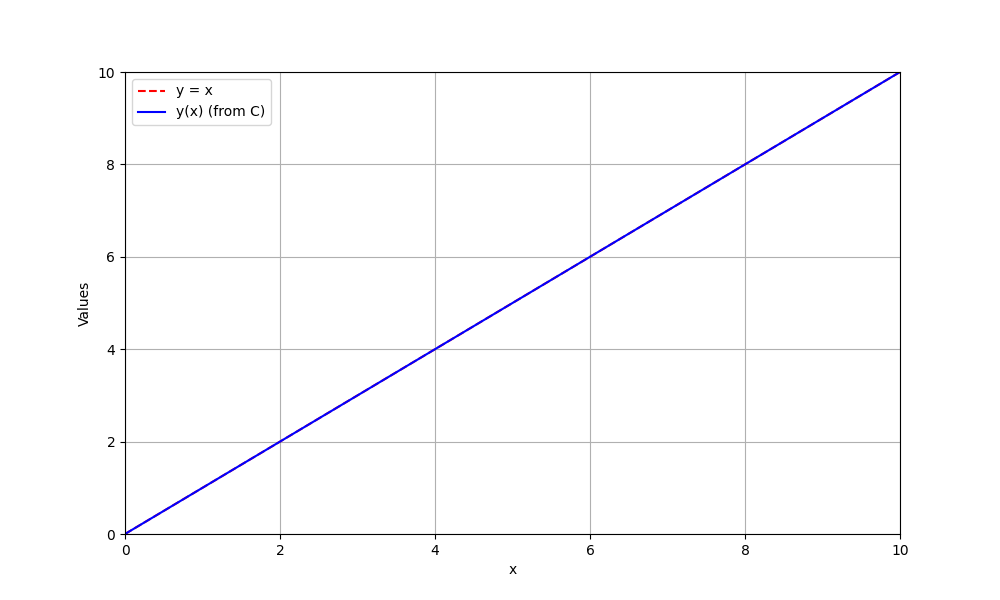
\includegraphics[width=\columnwidth]{fig.png}
		\caption{Solution of the given function}
		\label{stemplot}
	\end{figure}



\end{document}
